\documentclass[11pt]{article}
% Кодировка и язык
\usepackage[utf8]{inputenc}           % Кодировка исходного файла (UTF-8)
\usepackage[T2A]{fontenc}             % Кодировка шрифтов для кириллицы
\usepackage[english,russian]{babel}   % Локализация: русские названия, переносы

% Поиск в PDF
\usepackage{cmap}                     

% Поля страницы
\usepackage{geometry}
\geometry{left=2cm, right=2cm, top=2cm, bottom=2cm}

% Математика
\usepackage{amsmath, amssymb, amsthm} % Базовые пакеты для математики
\usepackage{mathtools}                % Расширение amsmath (доп. символы и окружения)

% Картинки
\usepackage{graphicx}                 % Вставка картинок (\includegraphics)
\graphicspath{{pictures/}}            % Путь к папке с картинками
\usepackage{float}                    % Позволяет использовать [H] для жёсткого позиционирования
\usepackage{wrapfig}                  % Обтекание текста вокруг картинок

% Таблицы
\usepackage{array}                    % Расширенные возможности для таблиц
\usepackage{booktabs}                 % Красивые таблицы (\toprule, \midrule, \bottomrule)
\usepackage{multirow}                 % Объединение строк в таблицах
\usepackage{tabularx}                 % Таблицы с автоматической шириной колонок
\usepackage{ragged2e}                 % Улучшенное выравнивание (используется в tabularx)

% Списки
\usepackage{enumitem}                 % Гибкая настройка списков (itemize, enumerate)

% Колонтитулы
\usepackage{fancyhdr}                 

% Гиперссылки
\usepackage{xcolor}                   % Работа с цветами
\usepackage{hyperref}                 % Гиперссылки, оглавление, перекрёстные ссылки

% Умные ссылки
\usepackage{cleveref}                 

% Типографика
\usepackage[expansion=false]{microtype}                % Улучшает переносы и межсловные расстояния

% Подписи к картинкам и таблицам
\usepackage{caption}                  % Настройка подписей (шрифт, отступы)

% Рисование схем и графиков
\usepackage{tikz}                     % Рисование схем, графиков, диаграмм
\usepackage{pgfplots}                 % Построение графиков функций (на основе tikz)
\pgfplotsset{compat=newest}           % Версия совместимости pgfplots

% Алгоритмы и код
\usepackage{algorithm}                % Окружения для алгоритмов
\usepackage{algorithmic}              % Синтаксис для алгоритмов
\usepackage{listings}                 % Вставка кода с подсветкой синтаксиса


% Настройка нумерации секций и подсекций
\renewcommand{\thesection}{\arabic{section}}                   
\renewcommand{\thesubsection}{\thesection.\arabic{subsection}} 


% Настройка списков: убираем лишние отступы слева
\setlist[itemize]{leftmargin=*}
\setlist[enumerate]{leftmargin=*}


% Определение окружений для теорем, лемм, определений и т.д.
% Нумерация привязана к номеру секции
\newtheorem{theorem}{Теорема}[section]
\newtheorem{definition}{Определение}[section]
\newtheorem{remark}{Замечание}[section]
\newtheorem{lemma}{Лемма}[section]
\newtheorem{example}{Пример}[section]
\newtheorem{consequence}{Следствие}[section]
\newtheorem{algorithmm}{Алгоритм}
\newtheorem{question}{Вопрос}[section]
\newtheorem{answer}{Ответ}[section]
\newtheorem{statement}{Утверждение}[section]


% Определение цветов
\definecolor{pblue}{rgb}{0.13,0.13,1}    
\definecolor{pgreen}{rgb}{0,0.5,0}       
\definecolor{pred}{rgb}{0.9,0,0}         
\definecolor{pgrey}{rgb}{0.46,0.45,0.48}

\DeclareMathOperator{\SAT}{SAT}
\DeclareMathOperator{\tSAT}{3-SAT}
\DeclareMathOperator{\tCOL}{2COL}
\DeclareMathOperator{\trCOL}{3COL}
\DeclareMathOperator{\VERTEXCOVER}{VERTEXCOVER}
\DeclareMathOperator{\DHAMPATH}{DHAMPATH}
\DeclareMathOperator{\CLIQUE}{CLIQUE}
\DeclareMathOperator{\INDSET}{INDSET}
\DeclareMathOperator{\Poly}{P}
\DeclareMathOperator{\NotDet}{N}
\DeclareMathOperator{\NP}{NP}
\DeclareMathOperator{\poly}{poly}

\newcommand{\lectureNumber}{5}
\newcommand{\lectureTitle}{Задачи $\VERTEXCOVER$, $\CLIQUE$ и $\INDSET$. $\NP$-полнота задач $\trCOL$ и $\DHAMPATH$.}
\newcommand{\courseName}{Формальные языки и сложность вычислений}
\newcommand{\semester}{3 семестр, 2026/2027 уч. год}

\pagestyle{fancy}
\fancyhf{}
\fancyhead[L]{Красота в глазах смотрящего}
\fancyhead[R]{\thepage}
\setlength{\headheight}{15pt}

\hypersetup{
    colorlinks=true,
    linkcolor=blue!70!black,
    citecolor=blue!70!black,
    filecolor=blue!70!black,
    urlcolor=blue!70!black,
}

\begin{document}


\begin{titlepage}
    \centering
    
    {\large Московский физико-технический институт \par}
    {\large Высшая школа программной инженерии \par}
    \vspace{2cm}

    {\Large \textbf{\courseName} \par}
    {\large \semester \par}
    
    \vspace*{\fill}

    {\Huge \textbf{Лекция \lectureNumber} \par}
    {\Huge \textbf{\lectureTitle} \par}
    
    \vspace*{\fill}
    
    {\large Лектор: Зухба Анастасия Викторовна \par}
    {\large Автор: \href{https://t.me/ceagest}{Юра} \par}

\end{titlepage}

\pagenumbering{arabic}

\section{Немного воспоминаний с семинаров}

Рассмотрим следующие три задачки:

\[\VERTEXCOVER = \{(G, k) \; | \; \text{в графе } G \text{ есть вершинное покрытие размера } k\}\]
\[\CLIQUE = \{(G, k) \; | \; \text{в графе } G \text{ есть клика из } k \text{ вершин}\}\]
\[\INDSET = \{(G, k) \; | \; \text{в графе } G \text{ есть независимое множество из } k \text{ вершин}\}\]
Убедимся, что они полиномиально сводятся друг к другу. Действительно:

\begin{enumerate}
    \item ($\CLIQUE \leq_{p} \INDSET$): По экземпляру $(G, k)$ задачи $\CLIQUE$ построим пару $(\overline{G}, k)$. Если в графе есть клика размера $k$, то в его дополнении есть независимое множество этого размера, и наоборот (смотрим в определение, рисуем себе пару примерчиков, и убеждаемся в этом).
    \item ($\VERTEXCOVER \leq_{p} \CLIQUE$): По экземпляру $(G, k)$ задачи $\VERTEXCOVER$ построим пару $(\overline{G}, \left\lvert V \right\rvert - k)$. Если в графе есть вершинное покрытие размера $k$, то оставшиеся вершины этого графа образуют независимое множество из $\left\lvert V \right\rvert - k$ вершин. Следовательно, в дополнении этого графа это независимое множество становится кликой того же размера, и наоборот.
    \item ($\INDSET \leq_{p} \VERTEXCOVER$): По экземпляру $(G, k)$ задачи $\INDSET$ построим пару $(G, \left\lvert V \right\rvert - k)$. Если в графе есть вершинное покрытие размера $k$, то оставшиеся вершины этого графа образуют независимое множество из $\left\lvert V \right\rvert - k$ вершин.
\end{enumerate} \leavevmode
\\
Также на семинарах доказывали сводимость $\tSAT \leq_{p} \INDSET$, которую я здесь естественно не стану воспроизводить. Таким образом, все эти милашки $\NP$-полные.

\section{Дорогу новому, или задачи о раскрасках графа}

Из курса алгоритмов все мы (так ведь? :)) помним чудесный $\text{BFS}$, который сразу даёт нам $\tCOL \in \Poly$. Но вот с тремя цветами, то есть с задачей $\trCOL$, всё куда сложнее... Напомню, кстати, как она выглядит:

\[\trCOL = \{G \; | \; \text{вершины графа } G \text{ можно правильно раскрасить в } 3 \text{ цвета}\}\]
Будем доказывать, что эта задача $\NP$-полная. Для этого начнём с доказательства её $\NP$-трудности. Будем сводить $\tSAT \leq_{p} \trCOL$. \\
Заметим, что для того, чтобы гарантировать цвет какой то вершины, нужно соединить её ребрами с двумя вершинами других цветов (конечно, в предположении, что раскраска правильная):

\begin{figure}[h]
\centering
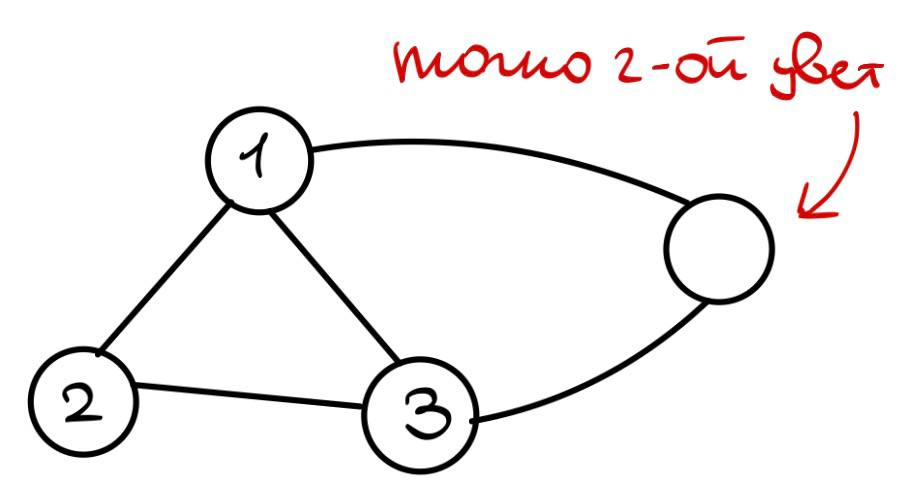
\includegraphics[width=0.5\linewidth]{третий цвет.jpg}
\end{figure} \leavevmode
\\
Пусть у нас есть формула вида:
\[(a \lor b \lor \overline{c}) \land (\overline{a} \lor b \lor d) \land (a \lor \overline{b} \lor d) \land (b \lor \overline{c} \lor \overline{d})\]
По ней мы будем строить граф.
\begin{enumerate}
    \item Каждой переменной и её отрицанию сопоставим по вершине, и соединим их ребром (так как никакая переменная не может быть истинна и ложна одновременно). \\
    В нашем случае получается нечто такое:
    \begin{figure}[h]
    \centering
    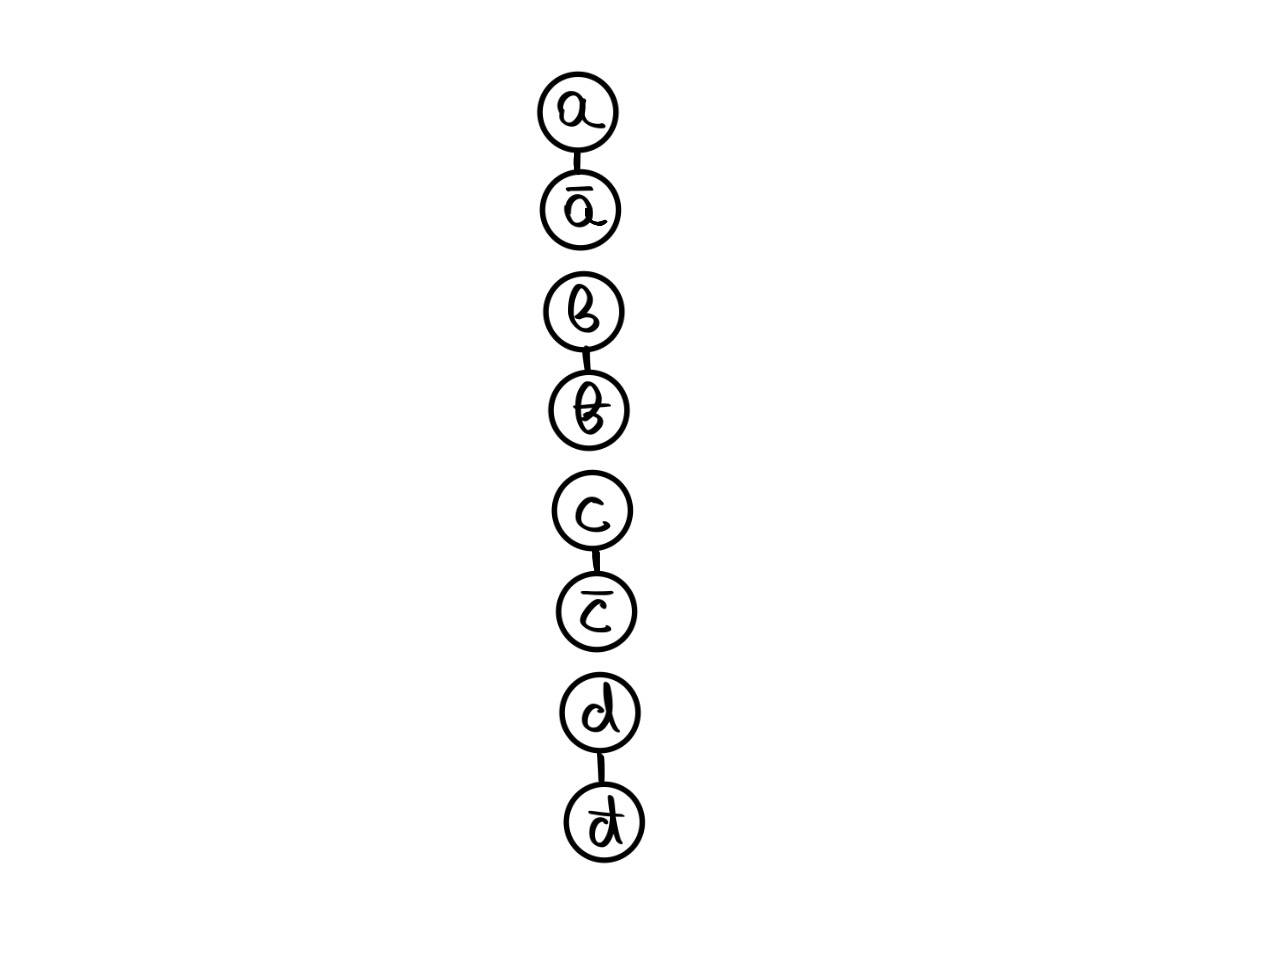
\includegraphics[width=0.7\linewidth]{литералы и отрицания.jpg}
    \end{figure}
    \item Добавим $3$ попарно связные вершины (соответствуют T, F и R, то есть мы как бы вводим два цвета под ложь и истину, и ещё один служебный), и все вершины литералов свяжем с R.
    \begin{figure}[h]
    \centering
    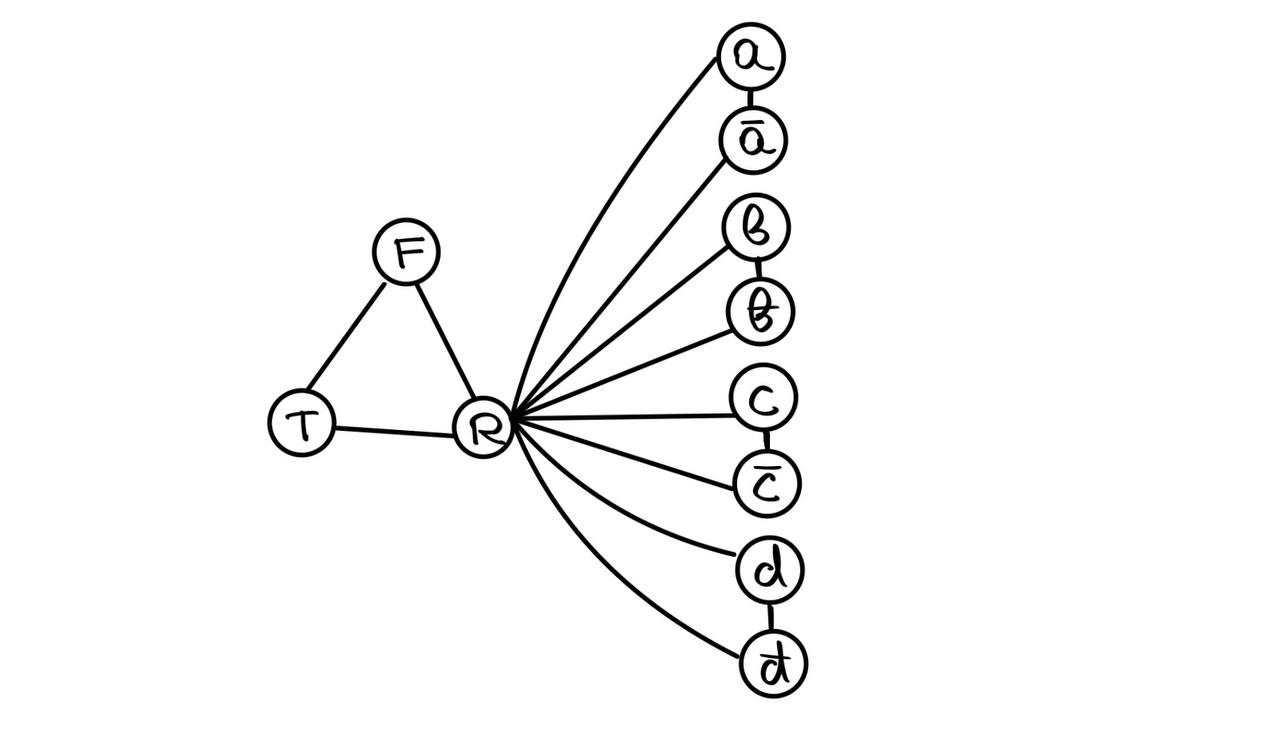
\includegraphics[width=0.7\linewidth]{добавили треугольник.jpg}
    \end{figure} \leavevmode
    \\
    Теперь рассмотрим вспомогательную конструкцию:
    \\
    \begin{figure}[h]
    \centering
    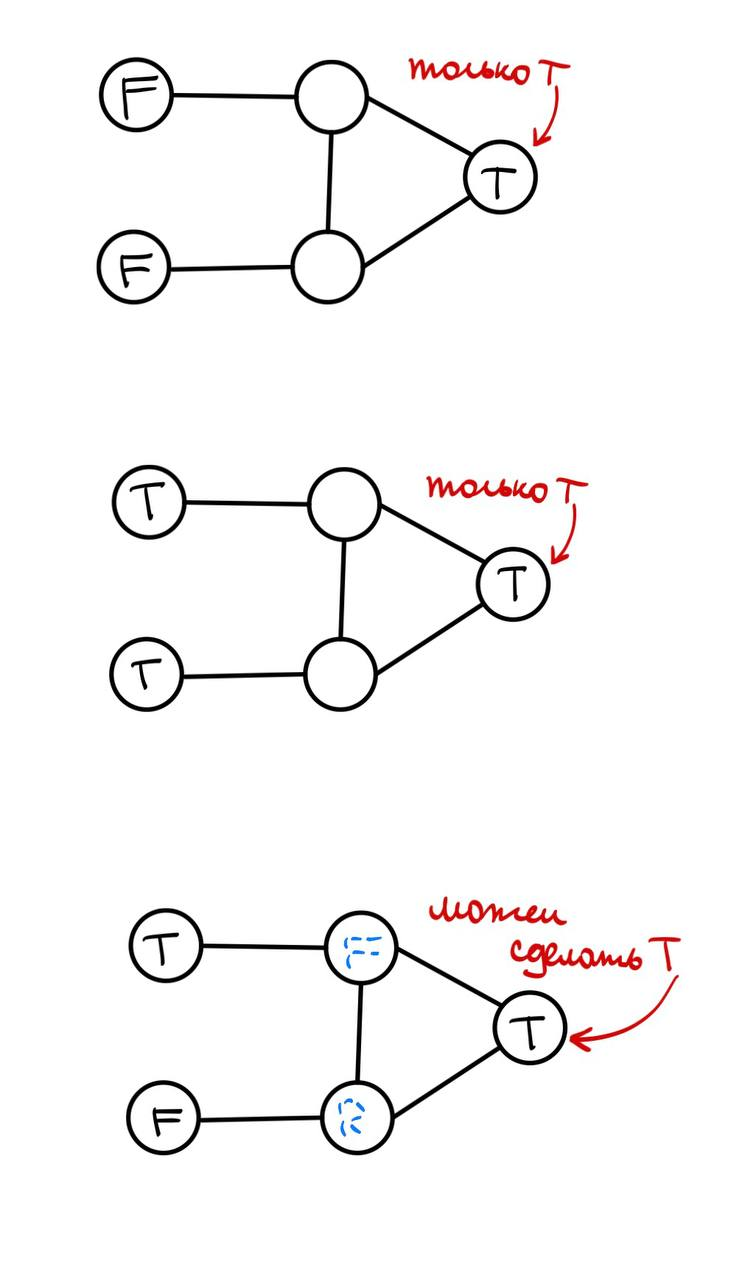
\includegraphics[width=0.4\linewidth]{три гаджета.jpg}
    \end{figure} \leavevmode
    \\
    Эти тайные знания пригодятся нам в третьем шаге.
    \item Для каждого дизъюнкта достроим \textit{гаджет} (некоторая странненькая дополнительная конструкция заданного вида):
    \begin{figure}[h]
    \centering
    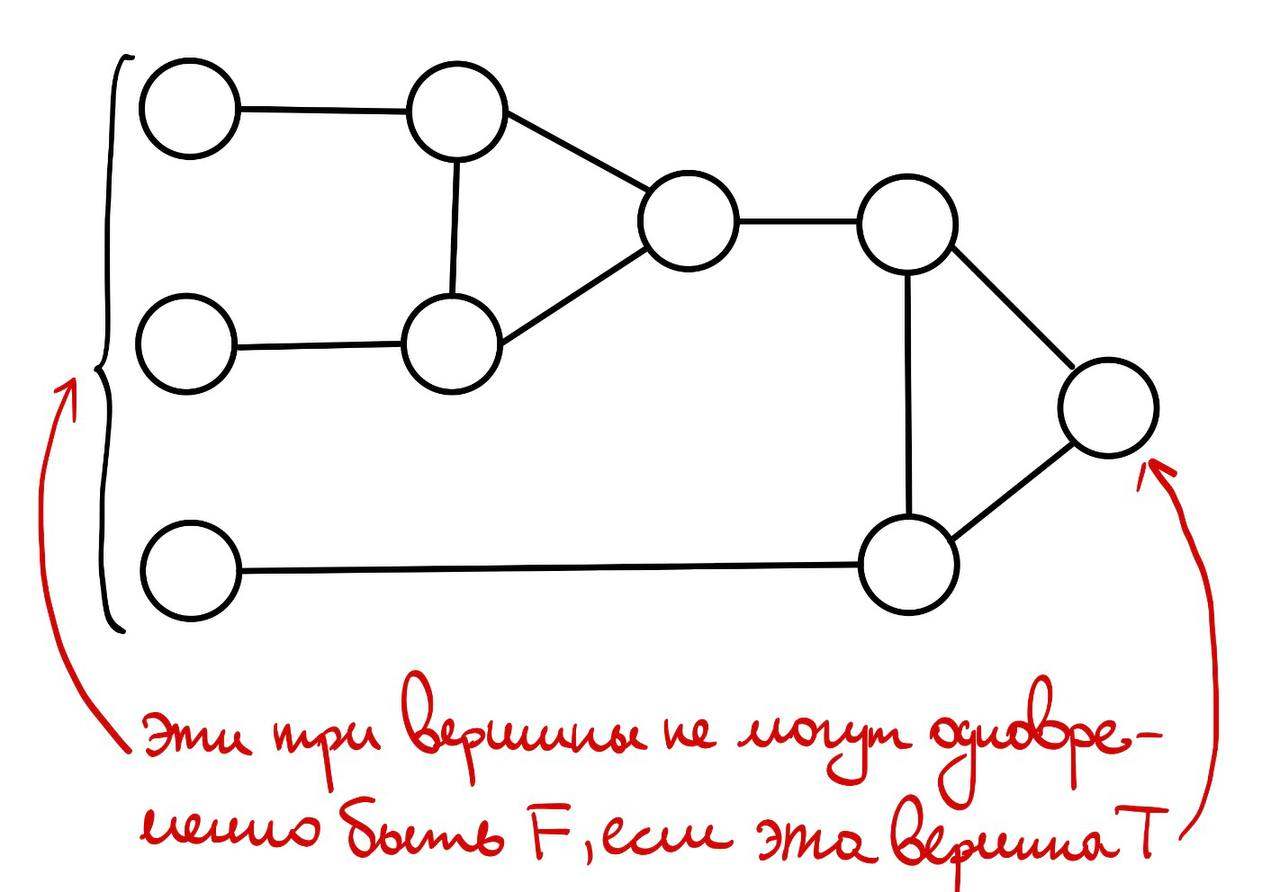
\includegraphics[width=0.45\linewidth]{гаджет.jpg}
    \end{figure} \leavevmode
    \\
    У нас получится что то такое (на рисунке нарисовал не все гаджеты, потому что и так страшно вышло):
    \\
    \begin{figure}[h]
    \centering
    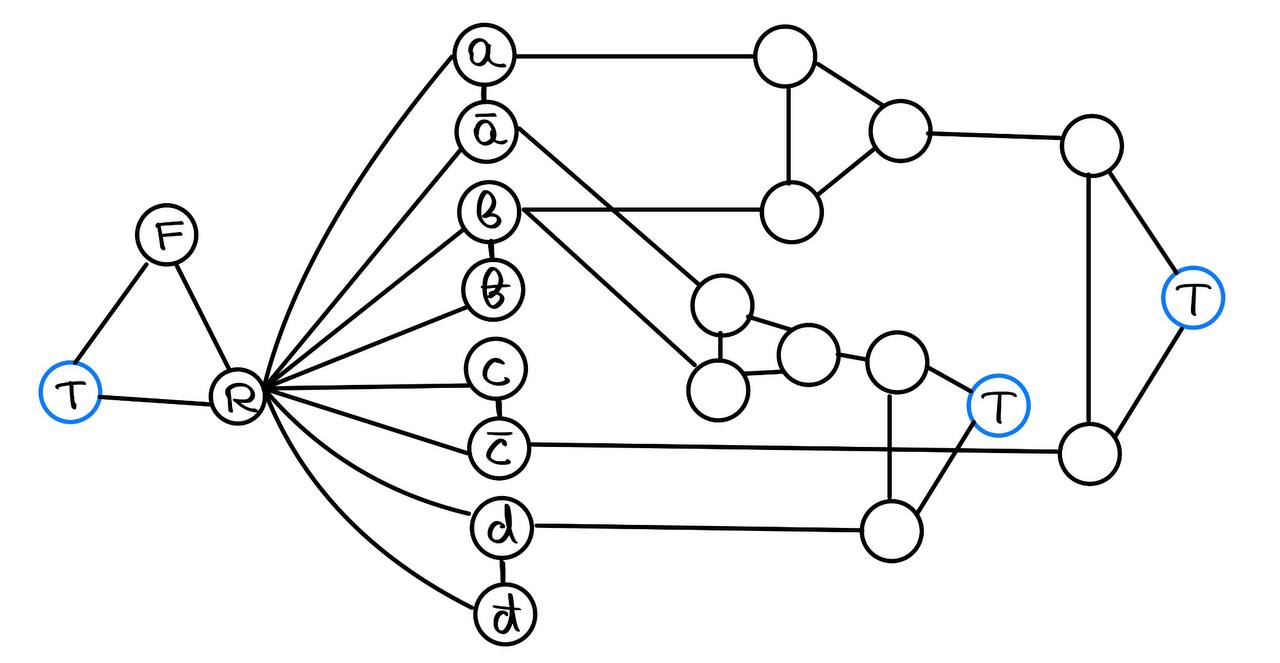
\includegraphics[width=0.89\linewidth]{страшная конструкция.jpg}
    \end{figure} \leavevmode
    \\ \\
    Чтобы не тянуть кучу рёбер в другой конец рисунка, вершина T обведена синим, дабы показать, что это всё одна и та же вершина.
\end{enumerate}
Ура, построение графа по формуле завершено. Теперь проверим, что всё хорошо со сводимостью. Действительно, для каждого дизъюнкта добавляется некоторое конечное фиксированное число вершин, а значит построение выполняется за полиномиальное время.
    При этом, если исходная формула была выполнима, то красим в соответствующие цвета наш граф, и получаем правильную раскраску в $3$ цвета. Если же построенный граф допускает раскраску в $3$ цвета, то из построения гарантируется, что литералы покрашены только в T или F, и никакие три литерала, лежащие в одном дизъюнкте, не могут быть одновременно F (свойство гаджета на картинке выше). Следовательно, получили выполняющий набор для исходной формулы. \\
    Таким образом, сводимость $\tSAT \leq_{p} \trCOL$ установлена, а значит $\trCOL$ является $\NP$-трудной задачкой. \\ 
    Принадлежность к $\NP$ увидеть совсем просто: достаточно в качестве сертификата брать раскраску $G$ в $3$ цвета. \\
    Итак, задача $\trCOL$ является $\NP$-трудной и лежит в $\NP$, а значит она $\NP$-полна, что мы и хотели.

\section{Гамильтоновость и друзья}

Итак, сформулируем всё это дружное семейство:
\[\text{DHAMPATH --- язык ориентированных графов } G \text{, содержащих гамильтонов путь}\]
\[\text{HAMPATH --- язык неориентированных графов } G \text{, содержащих гамильтонов путь}\]
\[\text{DHAMPATH-ST --- } (G, s, t) \; | \text{ ориентированный граф } G \text{ содержит гамильтонов путь из } s \text{ в } t\]
\[\text{HAMPATH-ST --- } (G, s, t) \; | \text{ неориентированный граф } G \text{ содержит гамильтонов путь из } s \text{ в } t\]
\[\text{DHAMCYCLE --- язык ориентированных графов } G \text{, содержащих гамильтонов цикл}\]
\[\text{HAMCYCLE --- язык неориентированных графов } G \text{, содержащих гамильтонов цикл}\]
\[\text{TSP --- } (G, w, s, t, L) \; | \text{ в полном взвешенном графе } (G, w) \text{ есть путь из } s \text{ в } t \text{, }\]
\[\text{ проходящий по всем вершинам графа, общего веса не более } L\]
Как и в самом первом блоке, все они полиномиально сводятся друг к другу. Доказательство, конечно же, отдаётся на откуп семинарам и здравому смыслу. Наша цель сейчас будет состоять в том, чтобы показать $\NP$-полноту какой то одной из них. \\
Будем доказывать, что $\tSAT \leq_{p} \text{DHAMPATH}$. Рассмотрим формулу вида:
\[\underbrace{(a \lor \overline{b} \lor c) \land (a \lor b \lor \overline{d}) \land \ldots}_{m \text{ дизъюнктов и } k \text{ переменных}}\]

\begin{enumerate}
    \item Для каждой переменной добавим гаджет:
    \begin{figure}[h]
    \centering
    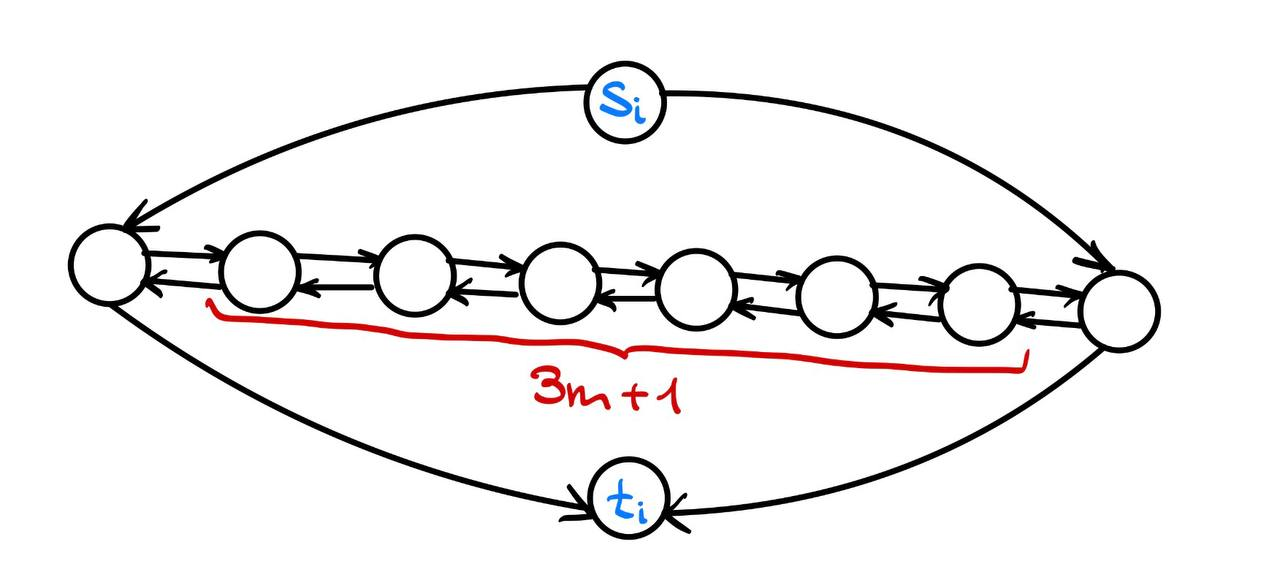
\includegraphics[width=0.7\linewidth]{ещё один гаджет.jpg}
    \end{figure} \leavevmode
    \\
    Если рассматривать эту конструкцию как отдельный граф, то в нём, очевидно, есть лишь два гамильтоновых пути.
    \item Соединим этих товарищей "подряд": вершину $t_i$ с вершиной $s_{i + 1}$. Пусть также $s_1 = s$, $t_k = t$.
    \item Для каждого дизъюнкта под номером $i$ заведём вершину $C_i$, $i = 1, \ldots, m$. \\
    Из $3m + 1$ вершины тех, которые имеют номера $1, 4, 7, \ldots, 3m + 1$, больше ни с чем не соединяем. \\
    Если переменная $x$ входит в дизъюнкт $n$ без отрицания, то в гаджете берём вершины $3n$ и $3n - 1$ и проводим рёбра:
    \begin{figure}[h]
    \centering
    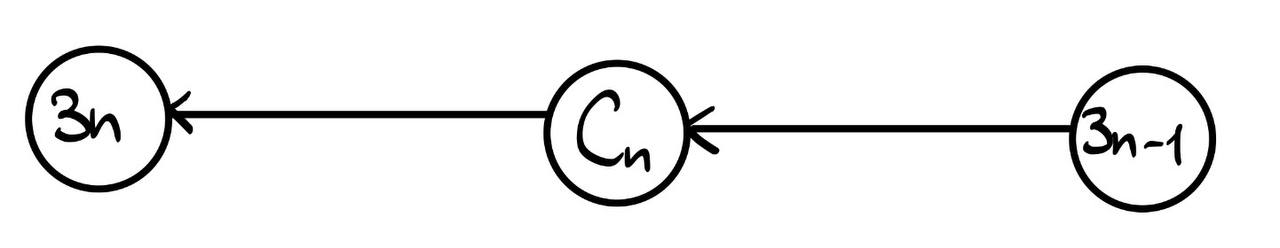
\includegraphics[width=0.6\linewidth]{первый кейс.jpg}
    \end{figure} \leavevmode
    \\
    Если же вершина $x$ входит в дизъюнкт $n$ с отрицанием, то:
    \begin{figure}[h]
    \centering
    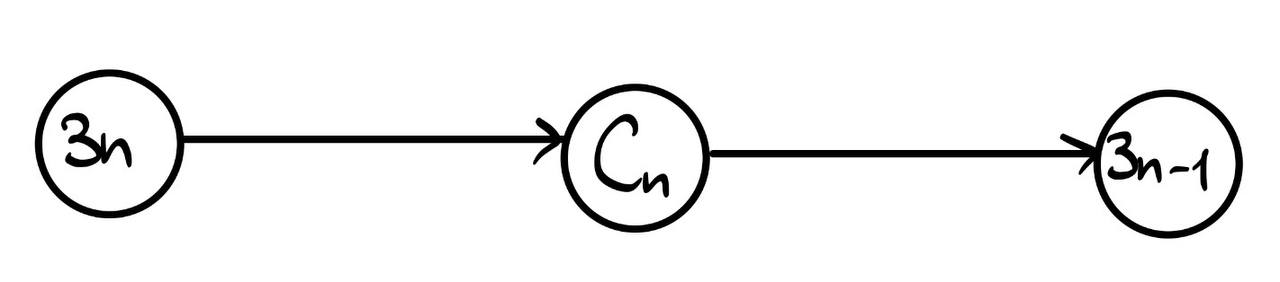
\includegraphics[width=0.6\linewidth]{второй кейс.jpg}
    \end{figure}
\end{enumerate}
Победа, мы снова построили граф по формуле. Теперь неплохо было бы понять, что всё это вообще значит. \\
Здесь кроется очень классная идея: истина и ложь определяются направлениями. Положительным для нас будет направление вправо, смотря из левой выходящей из $s_i$ стрелки, а оставшееся будет отрицательным. Проходя вдоль положительного направления по гаджету, для которого проведены соответствующие ребра в дизъюнкт $C_n$ в случае, когда переменная входит в $C_n$ без отрицания, по построению мы пройдём через $C_n$, минуя какое то ребро по пути вправо вдоль гаджета, и тем самым обращаем $C_n$ в истину. \\
\begin{figure}[h]
\centering
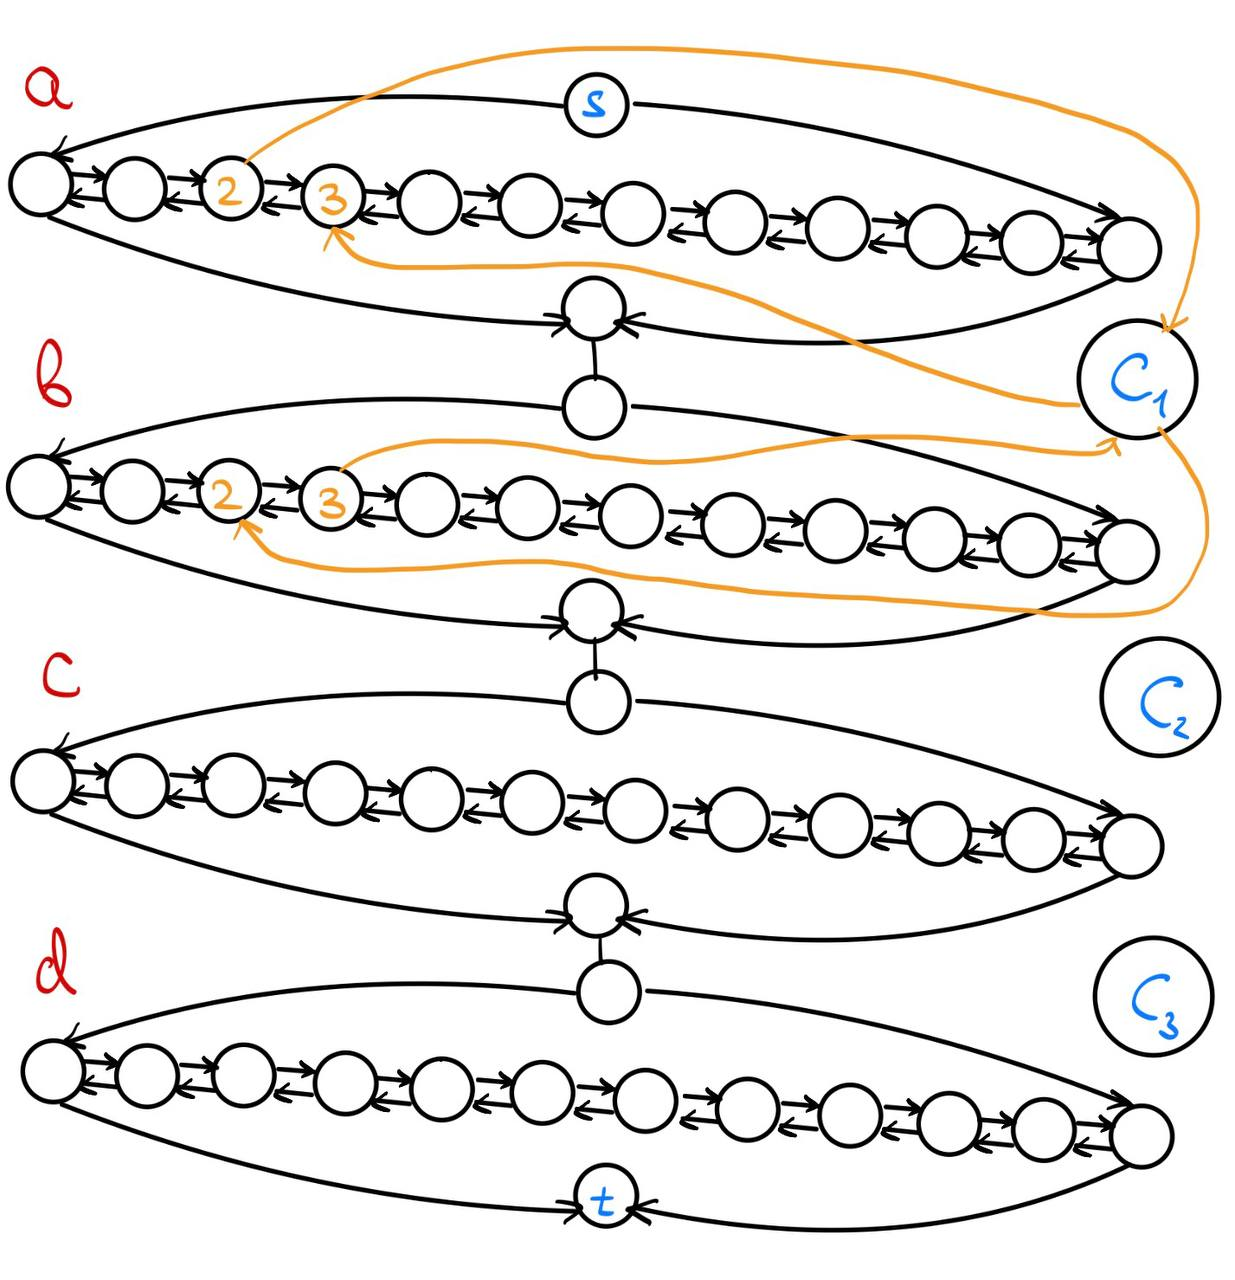
\includegraphics[width=0.7\linewidth]{огромный пример.jpg}
\caption{Пример при $m = 3$, $k = 4$}
\end{figure} \leavevmode
\\
Пусть исходная формула выполнима. Рассмотрим её выполняющий набор. Пусть, для примера, 
\[a = 1, b = 0, c = 1, \ldots\]
Тогда гаджеты, соответствующие переменным $a$ и $c$, будут обходиться в положительном направлении, а гаджет, соответствующий переменной $b$ --- в отрицательном. В первом дизъюнкте первый обратившийся в истину литерал есть $a$ (смотрим на исходную формулу). Следовательно, в вершину $C_1$ мы будем приходить и уходить через гаджет, соответствующий $a$ (идём только через первый, остальные не трогаем). Продолжая рассуждать так и дальше, получим требуемый гамильтонов путь. \\
Обратно, если гамильтонов путь существует, то будем идти по нему, придавая переменным значения, соответствующие знаку обхода гаджета. Так как в силу структуры построенного графа мы обязаны пройти через каждую вершину типа исток и сток, то всем переменным будут определены некоторые значения. При этом в каждой вершине, соответствующей дизъюнктам, мы тоже побываем ровно один раз, и сделаем это из гаджета в процессе обхода такого знака, что дизъюнкт обратится в истину при построенном наборе значений переменных. Следовательно, исходная формула будет выполнимой. \\
Осознав, что построение такого графа по формуле очевидно выполняется за полином, завершаем доказательство требуемой сводимости. \\
Таким образом, задачка $\text{DHAMPATH}$ является $\NP$-трудной. При этом она принадлежит $\NP$ --- достаточно взять сертификатом набор вершин гамильтонова пути. Следовательно, эта задача $\NP$-полная, чего мы и добивались.

\begin{remark}
    При построении графа в гаджете мы берем вершины таким образом, что между любыми двумя парами соседних вершин, соединённых с дизъюнктом ребрами, была одна свободная вершина. Это делается для того, чтобы между дизъюнктами не было паразитных путей, существование которых очевидно помешало бы нам добиться эквивалентности при сводимости.
\end{remark}


\end{document}